% !TeX root = ../main.tex
% Add the above to each chapter to make compiling the PDF easier in some editors.

\chapter{Case Studies}\label{chapter:applications}
With the bond of art and technology, deepfakes are slowly redefining the state of
entertainment. Their ability to transform audio and visuals offers creators better
possibilities to create new types of content. From refining the quality of amateur
videos to colorizing black-and-white movies, deepfakes are reshaping the entertainment
and art industries.

However, as explored in this research, the rise of deepfakes also underscores the pressing
need for effective detection mechanisms. The tools discussed in this thesis have direct
implications for the case studies presented here, as they offer potential solutions
to the challenges posed by deepfakes in various sectors.


\section{Entertainment and Art}
Deepfakes are popular in many creative areas. For example, rapper Kendrick Lamar
used deepfake in the 2022 music video to take on the looks of celebrities. In the
renewed Star Wars series, deepfake technology was used to resurrect characters like
Princess Leia and Moff Tarkin, despite the original actors having passed away~\cite{motion-analysis}.

The emergence of deepfake detection tools can play an important role in ensuring the
integrity of content in the entertainment industry. For instance, tools that can swiftly
and accurately detect manipulated content can help filmmakers and artists ensure that
their work remains authentic and free from unauthorized alterations.

The real question is: Is deepfake technology a blessing or a curse for talent?
An actor can feature in global commercials or websites
without constant traveling or learning new languages. For instance, Synthesia\footnote{\url{https://www.synthesia.io/}}
did this with two commercials starring rapper Snoop Dogg. Instead of reshooting for a
rebranded commercial, they altered Snoop Dogg's mouth movements to match the new brand
name using deepfakes~\cite{wipo-magazine}.

One of the positive implications of deepfakes in the Arts industry is, for example, the Salvador
Dalí Museum introduced \textit{Dalí Lives}, a digital revival of the deceased artist
Salvador Dalí using deepfakes~\cite{salvador-dali, salvador-dali2}.
This allows visitors to interact with the artist, hearing tales from his life, and
even taking selfies. The Museum used an encoder-decoder deepfake technique, training encoders on Dalí's
images and footage. An actor resembling Dalí was then mapped with Dalí's features using
decoders (\autoref{dali-youtube}).

\begin{figure}[ht]
	\centering
	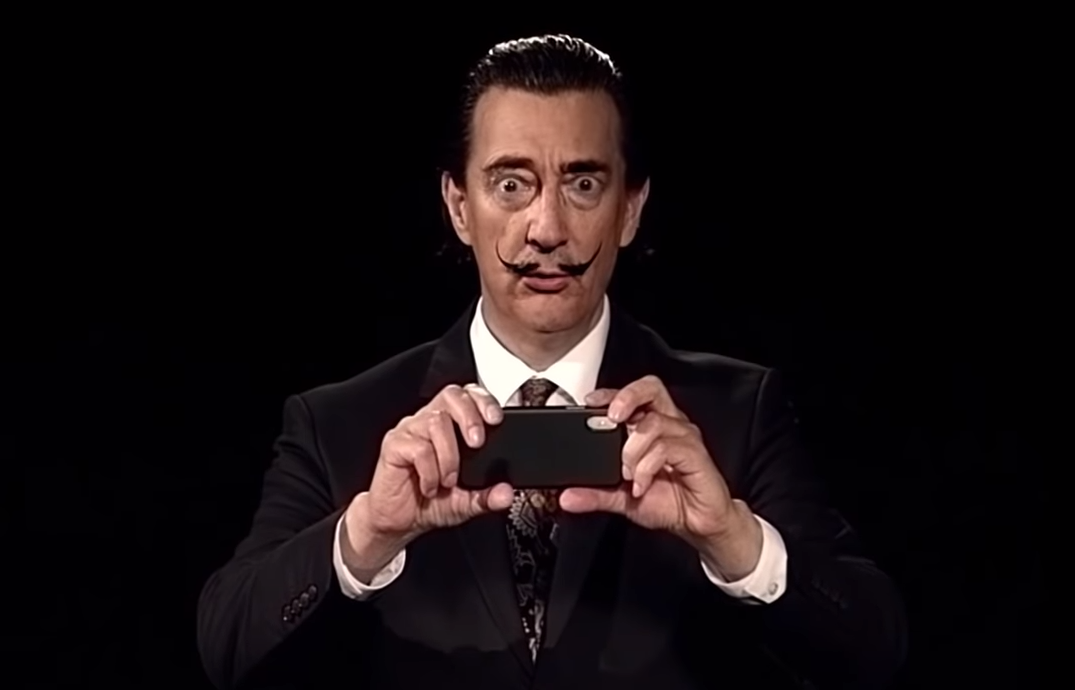
\includegraphics[width=0.61\columnwidth]{figures/dali}
	\caption{Screenshot taken from Dalí Lives~\cite{salvador-dali-youtube}.}\label{dali-youtube}
\end{figure}

Deepfakes, while being helpful and revolutionary, have notable weaknesses and can pose serious
threats. They have been misused for creating fake celebrity videos, committing fraud, and manipulating
political content, leading California to ban making political deepfakes during election
season in 2019~\cite{salvador-dali,california}. Such instances underscore the pressing need for
robust deepfake detection tools.


\section{Politics and Media}
With the rise of deepfakes in politics, the demand for effective detection tools
has also surged. Given the potential for deepfakes to influence public opinion,
especially during critical events like elections, there's an urgent need for tools
that can quickly and accurately identify manipulated content.

On the positive side of this context,
some political figures have used deepfakes in their campaigns for creative advertisements.
For instance, during the 2020 Delhi Legislative Assembly election in India, a deepfake video
of the president of India's \ac{BJP} party, Manoj Tiwari, spread on WhatsApp, as reported
by Vice~\cite{vice}. In this first-ot-its-kind campaign use, the original video of Tiwari speaking
English was changed to appear as if he spoke in Haryanvi, a Hindi dialect, targeting specific
voters. The \ac{BJP} collaborated with The Ideaz Factory to produce such deepfakes, aiming to
reach India's diverse linguistic audience. This particular deepfake reached reportedly 15 million
people across WhatsApp groups~\cite{india}.

Another case from politics involves a deepfake video created by Jordan Peele, where he
impersonated former U.S. President Barack Obama~\cite{peele,10.1145/3371409}. The video, widely
circulated on YouTube, depicted Obama making unexpected remarks, but was later revealed to be
manipulated with Peele's voice. When this video was analyzed using the Deepware deepfake
detection tool, it identified the content as a deepfake with a 93\% probability. This instance
highlights the importance of detection tools like Deepware in monitoring and verifying
political content.

\begin{figure}[ht]
	\centering
	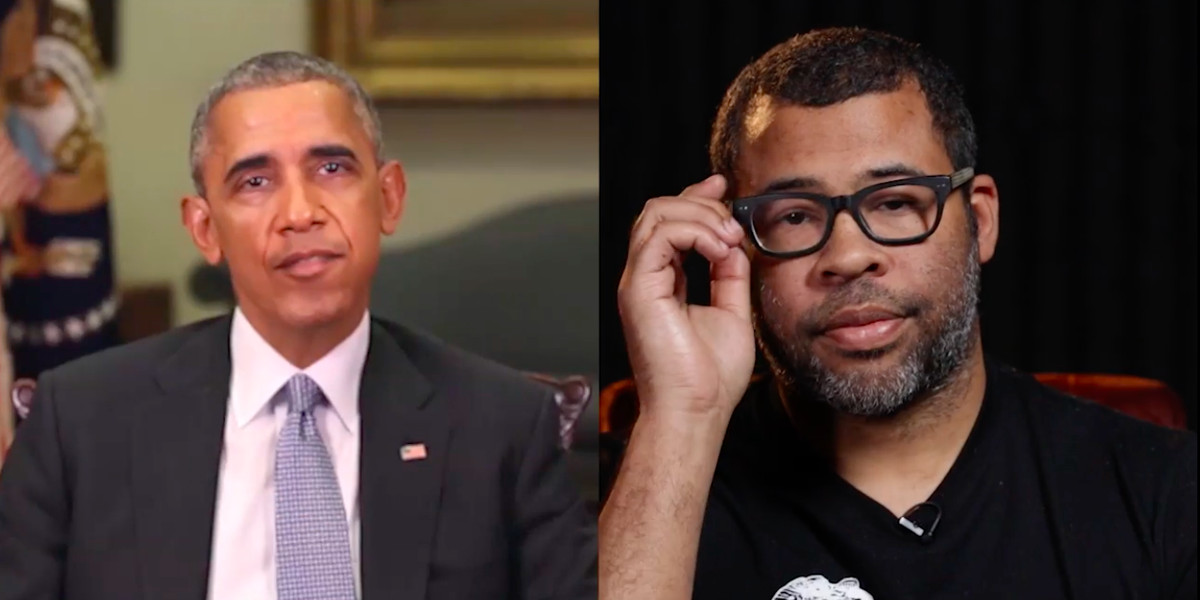
\includegraphics[width=0.8\columnwidth]{figures/obama}
	\caption{Screenshot taken from BuzzFeedVideo~\cite{peele}.}\label{obama-youtube}
\end{figure}

The risk of spreading misinformation in politics is high. There have been past
occurrences where fake videos were used to damage the reputation of political individuals.
Regulating political deepfakes is complex. While potential laws could aim to ban manipulated
content of politicians, they'd need exceptions to safeguard artistic and satirical content,
making implementation of those laws challenging due to the nature of satire and art~\cite{politics,vanity-fair}.
Promising solutions are emerging in the tech industry, as tech giants like Adobe and Microsoft,
alongside startups like Truepic\footnote{\url{https://truepic.com/}}, are developing tools for
authenticity verification.